\documentclass[osajnl,twocolumn,showpacs,superscriptaddress,10pt]{revtex4-1}


%PAQUETES<<<<<<<<<<<<<<<<<<<<<<<<<<<<<<<INICIO
\usepackage{dcolumn}% Align table %columns on decimal point
\usepackage{bm}% bold math
%
%Paquete de Idioma
\usepackage[spanish]{babel}
%
%Codificación Alfabeto
\usepackage[utf8]{inputenc}
%
%Codificación de Fuente
\usepackage[T1]{fontenc}
%
%Índice
\usepackage{makeidx}
%
%Gráficos3
\usepackage{graphicx}
\usepackage{subfig}
% \usepackage{longtable}
%\usepackage{xcolor} 
%
%Matemática
\usepackage{amsmath}
\usepackage{amsfonts}
\usepackage{amssymb}
%\usepackage{amstext} 
%
%Estilo de Página Numeración superior
%\pagestyle{headings}
%
%Hiperlinks \href{url}{text}
\usepackage[pdftex]{hyperref}
%
%Graficos y tablas
\usepackage{multirow}
%\usepackage{multicol}
\usepackage{float}
\usepackage{booktabs}
%
\decimalpoint
%\bibliographystyle{IEEEtran}
%\bibliography{IEEEabrv,mybibfile}
%
%
%PAQUETES<<<<<<<<<<<<<<<<<<<<<<<<<<<<<<<INICIO

\begin{document}
%SIGNOS
%TILDE -> \' <vocal>
%TEXTO_NEGRITA -> \textbf{<texto>}
%TEXTO_ITALICA -> \textit{<texto>}
%TEXTO_SUBRAYADO -> \underline{<texto>}

%TITTULO DEL ARTICULO
\title{\Huge IoT Proyecto Uno -  Banda Inteligente - Arquitectura de Computadores y Ensambladores 2 }
%AUTORES DEL ARTICULO

\author{\newline Airton Yelstin de León Obando (201602836) - Rol: Analítico}
\affiliation{Grupo No.15 - Universidad de San Carlos de Guatemala, Escuela de Ciencias y Sistemas
}%

\author{\newline Oswaldo Giovanni Cáceres Samayoa, (201314164) - Rol: Conectividad}%
\affiliation{Grupo No.15 - Universidad de San Carlos de Guatemala, Escuela de Ciencias y Sistemas
}%
\author{\newline Anggelo Santiago Son Mux, (201709502) - Rol: Conectividad}%
\affiliation{Grupo No.15 - Universidad de San Carlos de Guatemala, Escuela de Ciencias y Sistemas
}%
\author{\newline Byron Gerardo Castillo Gómez, (201700544) - Rol: Smart-APP}%
\affiliation{Grupo No.15 - Universidad de San Carlos de Guatemala, Escuela de Ciencias y Sistemas
}%
\author{\newline Cristian Alberto Suy Mejia, (201700918) - Rol: Infraestructura}%
\affiliation{Grupo No.15 - Universidad de San Carlos de Guatemala, Escuela de Ciencias y Sistemas
}%
\date{Febrero 2021}



%INICIO DE DOCUMENTO<<<<<<<<<<<<<<<<<<<<<<<<<<<<<<<<<
\begin{abstract}
\title {resumen}
En esta pr\'actica se pretende hacer uso del concepto de Internet de las Cosas ( IoT - Internet of Things ) aplicado a una banda inteligente. Esta banda se diseño de tal forma que sea capaz de transmitir informaci\'on de manera inmediata del estado del atleta al dispositivo de este mismo, lo anterior por medio de diferentes dispositivos electrónicos y sensores, adem\'as de un microcontrolador que recolecta la informaci\'on y la transmite a la nube. Todo lo anterior de manera que el usuario final tiene informaci\'on actualizada de su sobre su estado físico desde su dispositivo m\'ovil en cualquier momento y lugar.
\end{abstract}
\maketitle{}
\section{INTRODUCCIÓN}
Al hablar de introducir el concepto de IoT es este proyecto principalmente se habla de la importancia de recolectar datos a través de dispositivos y hacer uso de estos datos provenientes de cualquier objeto o situación de la vida diaria cuya utilidad aumenta significativamente al convertir estos datos en información relevante y de interés en su funcionamiento, de tal manera que este objeto expande sus funciones para las que fue originalmente creado. Esta banda inteligente fue diseñado para proveer una solución a aquellos atletas o deportistas que buscan mantener monitoreados sus signos vitales, medir magnitudes físicas relacionadas a la actividad física y tener control sobre las actividades que realizan. Debido a lo anterior esta banda inteligente es capaz de realizar medidas de actividad del ritmo cardiaco, nivel de oxigeno, temperatura y todo gracias a un conjunto de diferentes dispositivos y sensores instalados en al banda que funcionarán en conjunto, la banda inteligente tiene la capacidad obtener el estado de las atleta en tiempo real, mientras realiza sus actividades deportivas junto a ello puede obtener métricas de durante su actividad física, tales como: velocidad o distancia recorrida, además no solo podrá saber los números sobre su estado sino también podrá obtener gráficas e historial sobre su actividad reciente desde su dispositivo móvil, en cualquier lugar y en cualquier momento. La comunicación es posible a través tecnología Bluetooth integrada en la banda, una aplicación para dispositivos móviles con conexión a la banda e internet, de donde obtiene información proveniente de la nube y que se almacena en la nube.

\section{Prototipo de Diseño}
Considerando que el propósito de este objeto es monitorear el estado del usuario por medio de una banda para la muñeca, la cual estará integrada a un guante junto con los demás componentes, a continuación se puede apreciar un prototipo del objeto, observar Figura 1.


\begin{figure} [H] \centering 
\caption{Boceto de diseño}

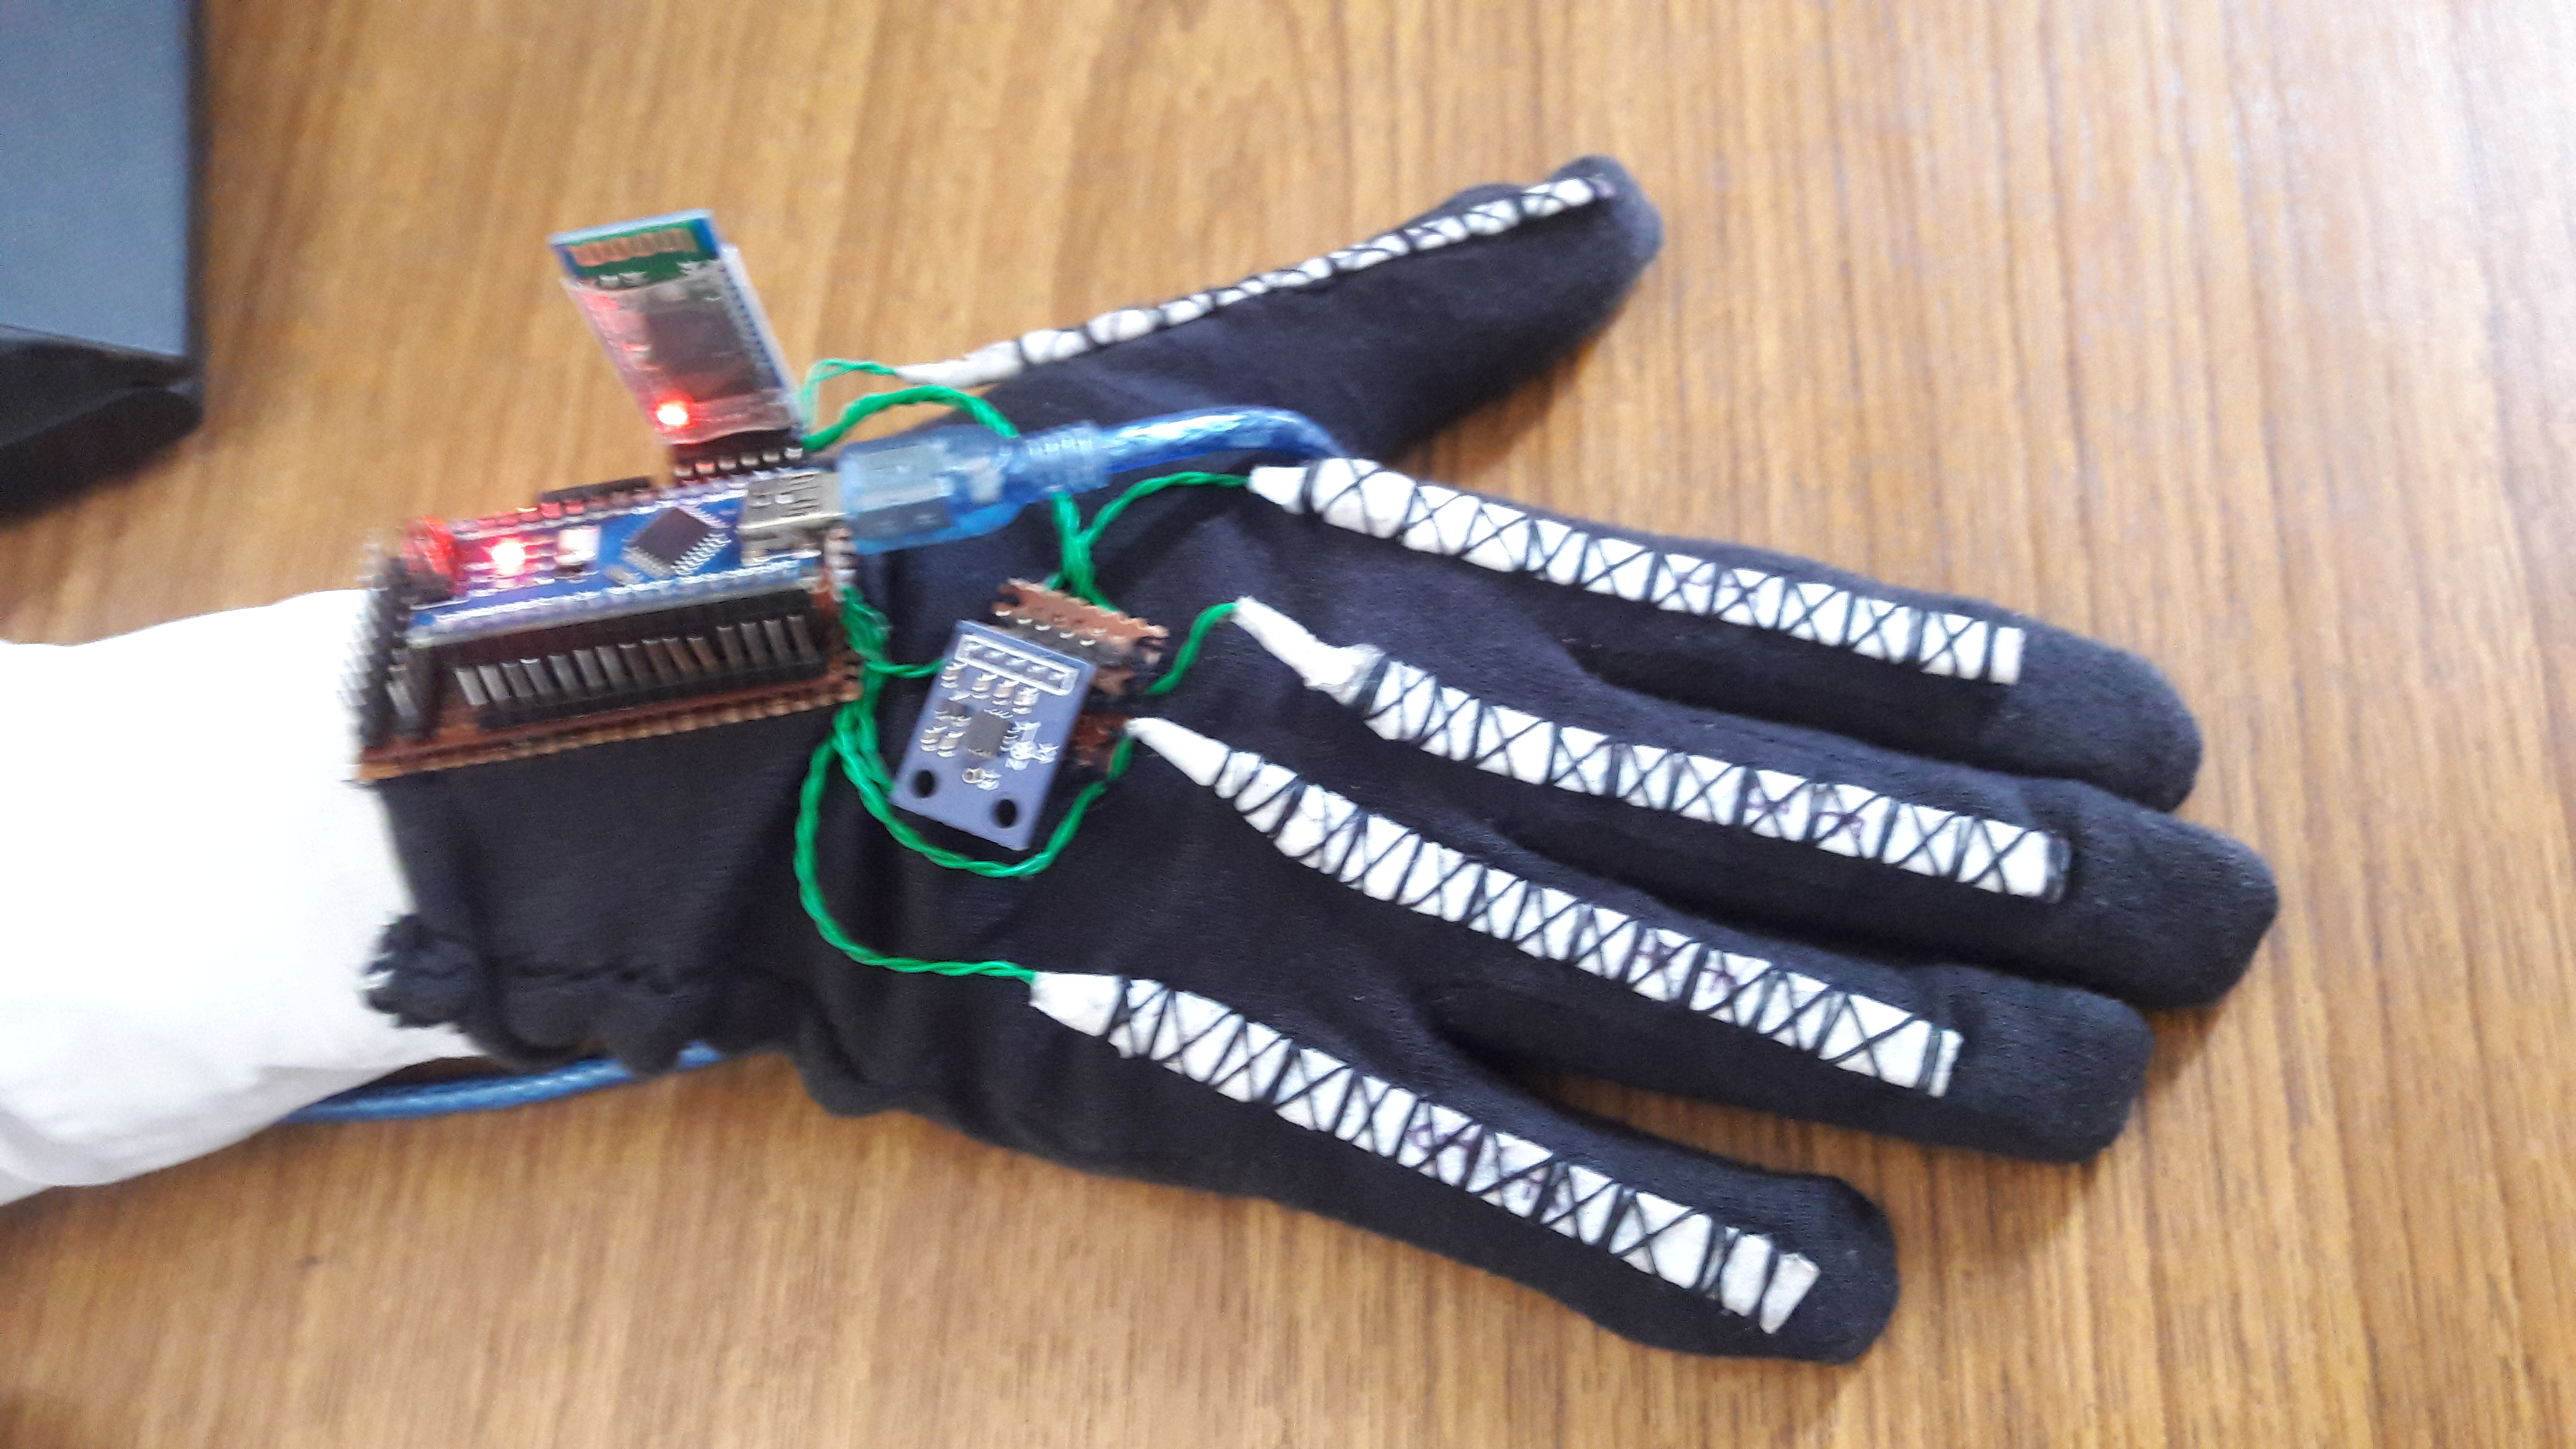
\includegraphics[width=0.5\textwidth]{prototipo.jpg} 
Considerando que los componentes de la banda inteligente serán integrados en un guante, se presenta una ilustración de como se disponen los componentes. 
\end{figure}

\section{Famework de Productos Inteligentes Conectados}
\subsection{Infraestructura del Producto}
\subsubsection{Hardware:}
\begin{itemize}
    \item[$\bullet$]\textbf{Guante} de lana para integrar los componentes de banda inteligente.
    \item[$\bullet$]Dispositivo de \textbf{Módulo Bluethoot, CH05} para conexión inalámbrica.
    \item[$\bullet$]\textbf{Arduino Mega}.
    \item[$\bullet$]\textbf{Cables} para conexiones.
    \item[$\bullet$]\textbf{Cautín} para realizar soldaduras.
    \item[$\bullet$]\textbf{Estaño.}
    \item[$\bullet$]\textbf{Buzzer} para indicar con un pitido el ritmo de las actividades físicas realizadas.
\end{itemize}
\subsubsection{Software}
    Se han diseñado y programado algoritmos y rutinas para la recolección constante de datos sobre el estado del cuerpo del usuario mientras este realiza actividades físicas, esto a través de diferentes sensores; las rutinas están diseñadas para que los datos obtenidos puedan ser información de utilidad y procurando eficiencia y simplicidad al momento de gestionar su recolección y transmisión. Estos datos son procesados con la ayuda de un microcontrolador ARDUINO, que a la vez envía dichos datos obtenidos al dispositivo móvil del usuario, para su posterior trasmisión al servidor y almacenamiento en la nube. la razón de haber elegido a ARDUINO fue debido a su capacidad y flexibilidad para realizar diversas tareas, costo accesible y su simple implementación.
    
\subsection{Sensores}
Para realizar las diferentes mediciones y lecturas sobre el estado corporal del usuario y sus actividades físicas se ha hecho uso de los siguientes sensores:
\begin{itemize}
    \item[$\bullet$]\textbf{Sensor de temperatura, LM34} para determinar la temperatura corporal del usuario.
    \item[$\bullet$]\textbf{Sensor de pulso y oxigeno, Max30102} para medir tanto el ritmo cardiaco como los niveles de oxigeno en la sangre del usuario mientras este realiza actividades físicas.
    \item[$\bullet$]\textbf{Acelerómetro} para medir magnitudes físicas, como velocidad y distancia alcanzadas por el usuario durante su rutina.
\end{itemize}
\subsection{Conexión}
    La comunicación a utilizar entre la banda inteligente y el dispositivo móvil del usuario será a través de conexión \textbf{Bluethoot} exclusivamente, el dispositivo arduino recolecta la información para ser transmitida desde el módulo \textbf{Bluethoot} a el dispositivo móvil, una vez los datos hayan sidos recolectados y normalizados estos serán enviados.  al dispositivo móvil que contara con conexión a internet y que a su vez realiza peticiones \textbf{HTTP} al servidor a través de una \textbf{API/REST}, que mediara el envío y recepción la información al dispositivo móvil del usuario, para posteriormente almacenar la información en una base de datos en al nube, específicamente a una base de datos de \textbf{Mongo DB.} Ver figura 2. \newline
\begin{figure} [H] \centering 
\caption{Representación de conexión}
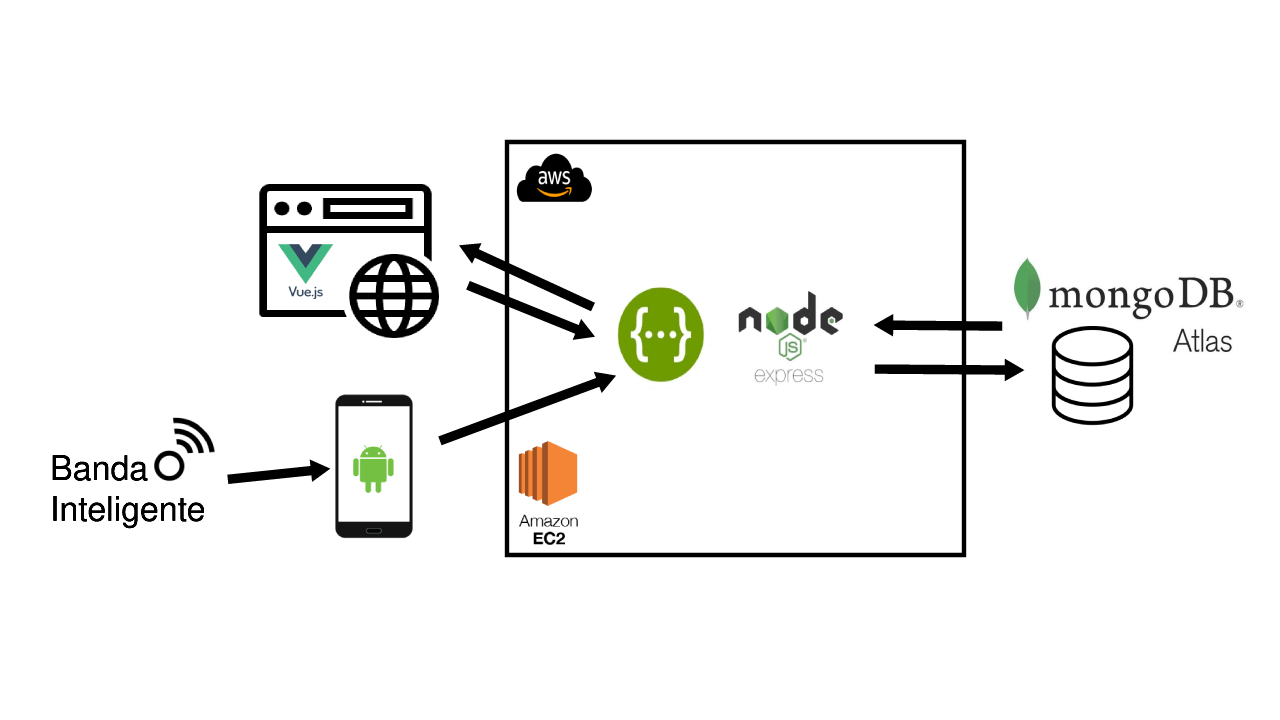
\includegraphics[width=0.55\textwidth]{Arquitectura.png} 
Puede apreciarse la dinámica de la conectividad, en la que los datos son enviados desde la banda al móvil, este a su vez realiza las peticiones HTTP a una API/REST, usando los servicio AWS (Amazon Web Services) de Armazón, para posteriormente almacenar la información en MongoDB.
\end{figure}

\subsection{Análisis}
    Durante una sesión de actividad física, la banda inteligente tomará lecturas sobre el estado corporal del usuario; también mide magnitudes físicas tales como la velocidad alcanza por el usuario y la distancia recorrida al inicio de la rutina, después de que los datos recolectados por los diferentes sensores sean normalizados, estos datos serán enviados al dispositivo móvil y posteriormente a la nube, donde los datos son convertidos en información relevante, útil y de interés para el usuario, entre ellas se tienen gráficas sobre las lecturas de niveles de oxigeno en la sangre, temperatura corporal y el ritmo cardiaco, además, en base a los datos recolectados se cuenta con un historial detallado sobre cada sesión de actividad, que serán catalogados e identificados con fecha y hora entre otras lecturas relevantes para el usuario, de tal forma que el dispositivo le de un agregado y limitarse a solamente tomar lecturas. Además se cuenta con la función de someterse a la prueba \textbf{Test Course Navette}, para ello se ejecutan diversos algoritmos para finalmente indicar los resultados obtenidos en la prueba basado en los datos recolectados Estas funcionalidades son descritas en las siguientes secciones.
    
\subsection{Aplicación Móvil}
    Ya que el usuario deberá tener acceso al estado de sus lecturas e historial de actividad de la banda inteligente en todo momento se ha de ha desarrollado una aplicación inteligente para dispositivos móviles. Esta aplicación es compatible con dispositivos que utilizan el Sistema Operativo \textbf{Android}, entre algunas de sus funcione más destacadas está el \textb{dash-board} con las mediciones de la actividad física del usuario, además una función integrada para realizar la prueba \textbf{Test Course Navette}, a continuación se pueden apreciar las pantallas que ilustran su funcionamiento:
    
\begin{figure} [H] \centering 
\caption{PANTALLA 1 ( Aplicación móvil )}
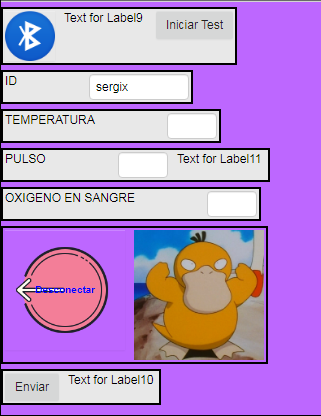
\includegraphics[width=0.45\textwidth]{PantallaPrincipal.png} 
\end{figure}

    Para poder realizar la conexión inalámbrica a través de  Bluethoot es necesario que el usuario ingrese su ID/Username para así verificar a quien le pertenecen los datos enviados.
    
\begin{figure} [H] \centering 
\caption{BLOCKS 1 ( Conexión Bluetooth )}
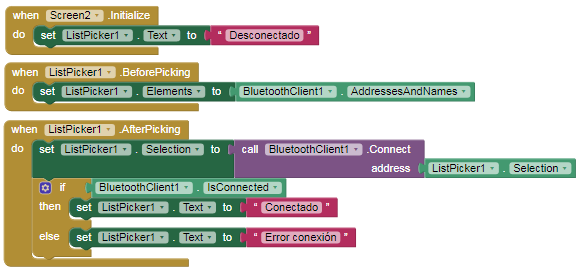
\includegraphics[width=0.5\textwidth]{ConexionBT.png} 
\end{figure}

\begin{figure} [H] \centering 
\caption{BLOCKS 2 ( Nueva Sesion )}
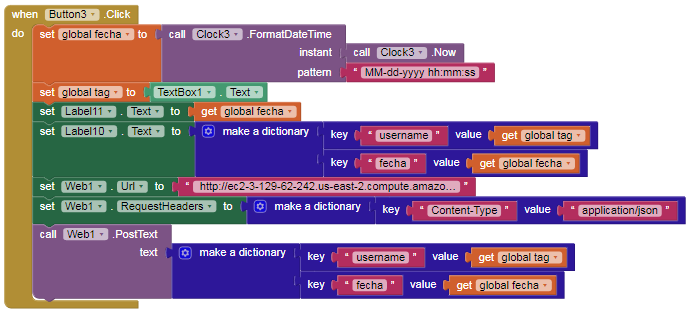
\includegraphics[width=0.5\textwidth]{NuevaSesion.PNG} 
\end{figure}

    Cada vez que la aplicación móvil recibe un nuevo paquete de provenientes de la banda inteligente, los datos de este se envían inmediatamente por medio de una API hacia una base de datos la cual contiene diferentes tablas donde se estarán guardando los datos que posteriormente serán procesados.
    
\begin{figure} [H] \centering 
\caption{BLOCKS 3 ( Envio de datos )}
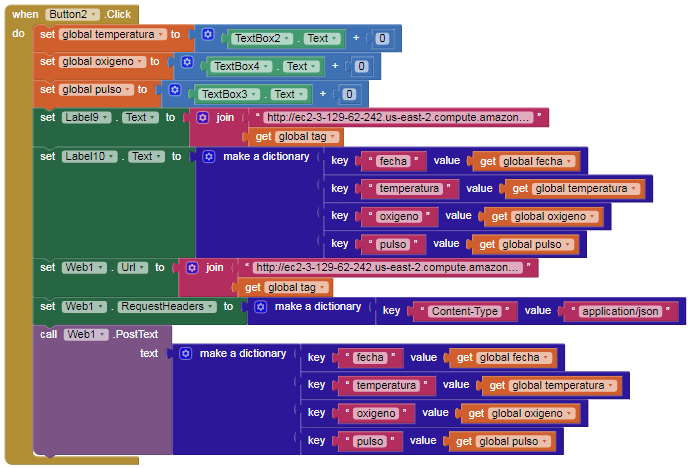
\includegraphics[width=0.5\textwidth]{EviarDatos.PNG} 
\end{figure}
\subsection{Smart APP: WEB}

    Al entrar en la aplicación web se desplegará un cuadro emergente de Login para que el usuario pueda ingresar sus credenciales y obtener acceso a la aplicación con sus respectivas lecturas, historial de actividad, gráfica de actividad física, además, en caso de no contar con un usuario este puede seleccionar la opción de Registrar para crear una nueva cuenta y hacer uso de las diferentes funciones disponibles.
    
\begin{figure} [H] \centering 
\caption{Figura 4: Login ( Página WEB )}
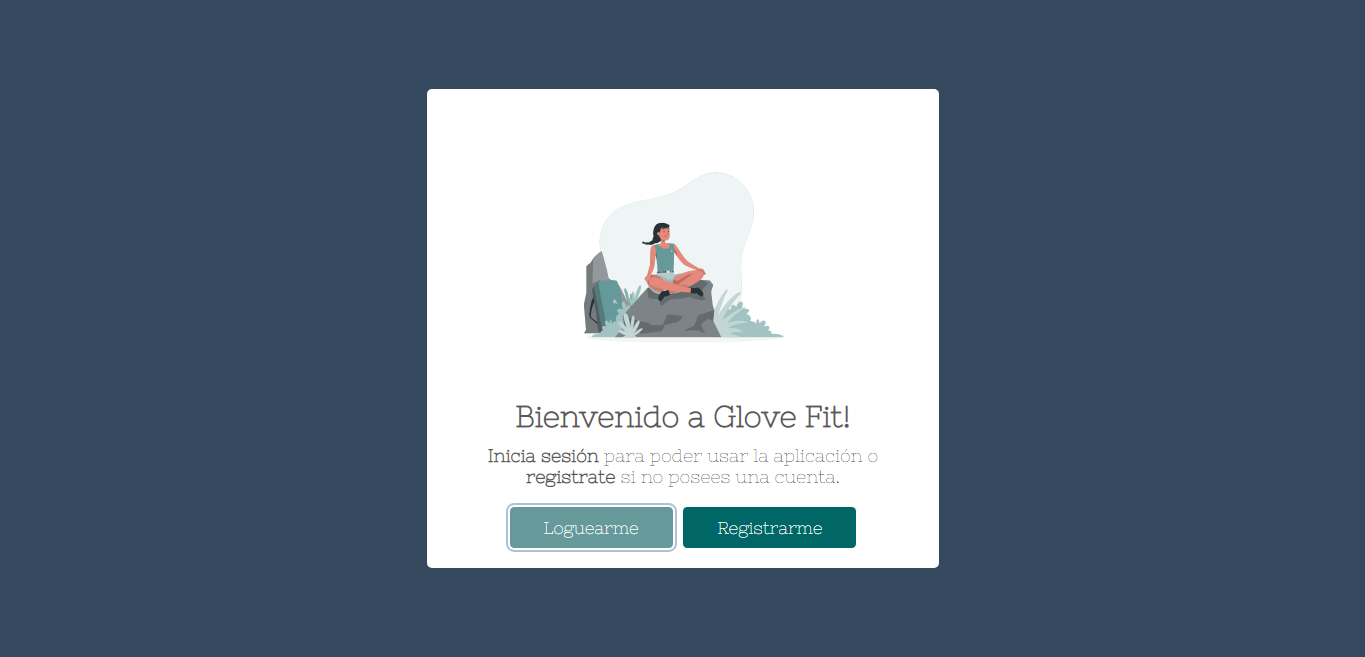
\includegraphics[width=0.45\textwidth]{Login.PNG}
\end{figure}

La pagina principal cuenta con 4 opciones:
\begin{itemize}
    \item[$\bullet$]Perfil 
    \item[$\bullet$]Ritmo Cardiaco
    \item[$\bullet$]Temperatura
    \item[$\bullet$]Oxigeno
\end{itemize}

\subsubsection{Perfil:}
    En esta sección se muestran la información personal del usuario junto con la información deportiva del usuario que inicio sección desde la aplicación web.
    
\begin{figure} [H] \centering 
\caption{Figura 5: Perfil ( Aplicación WEB )}
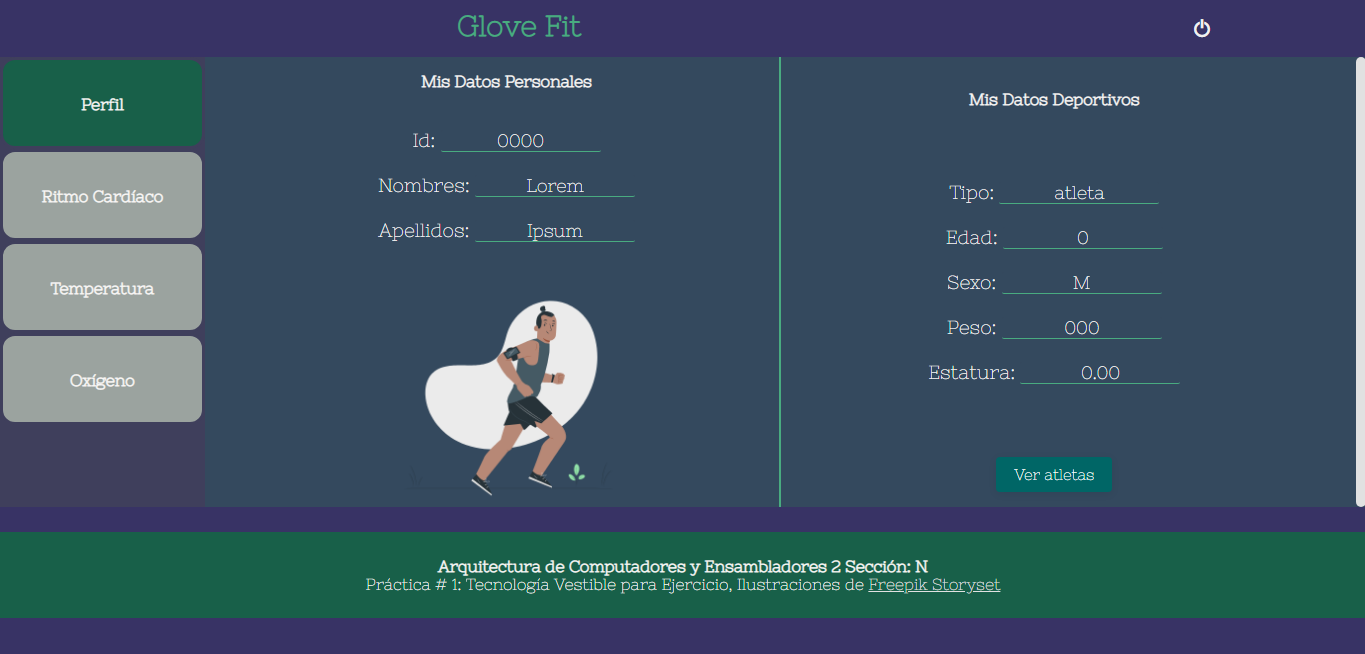
\includegraphics[width=0.45\textwidth]{Perfil.PNG}
\end{figure}

    Si el usuario ha ingresado a la aplicación web y es un usuario de tipo Coach, este podrá ver los datos de todos los atletas asignados a este, además, tiene la capacidad de monitorear el rendimiento de cada uno a través sus historiales.
    
\begin{figure} [H] \centering 
\caption{Figura 6: Coach-Atleta ( Página WEB )}
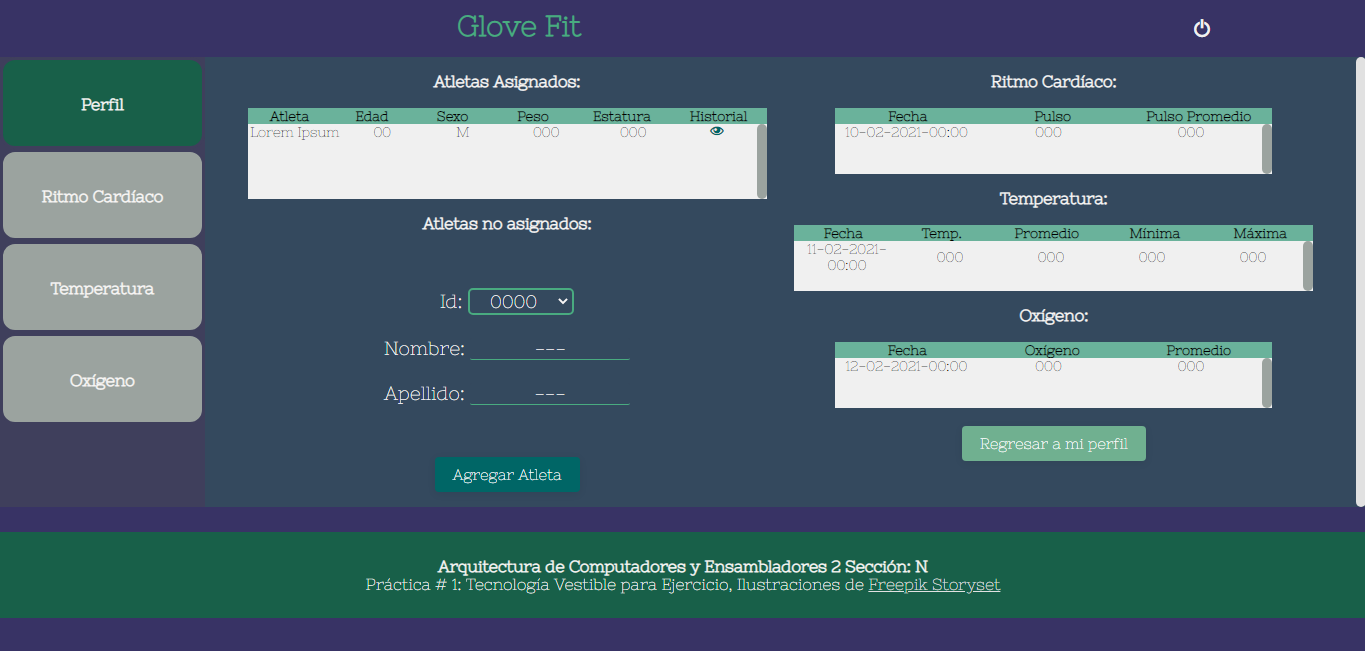
\includegraphics[width=0.45\textwidth]{CoachAtleta.PNG}
\end{figure}

\subsubsection{Ritmo Cardiaco:}
    En esta sección se muestra el control de ritmo cardiaco e indicadores de pulso en tiempo real provenientes de la banda inteligente integrada en el guante.
    
\begin{figure} [H] \centering 
\caption{Figura 6: Ritmo Cardiaco ( Página WEB )}
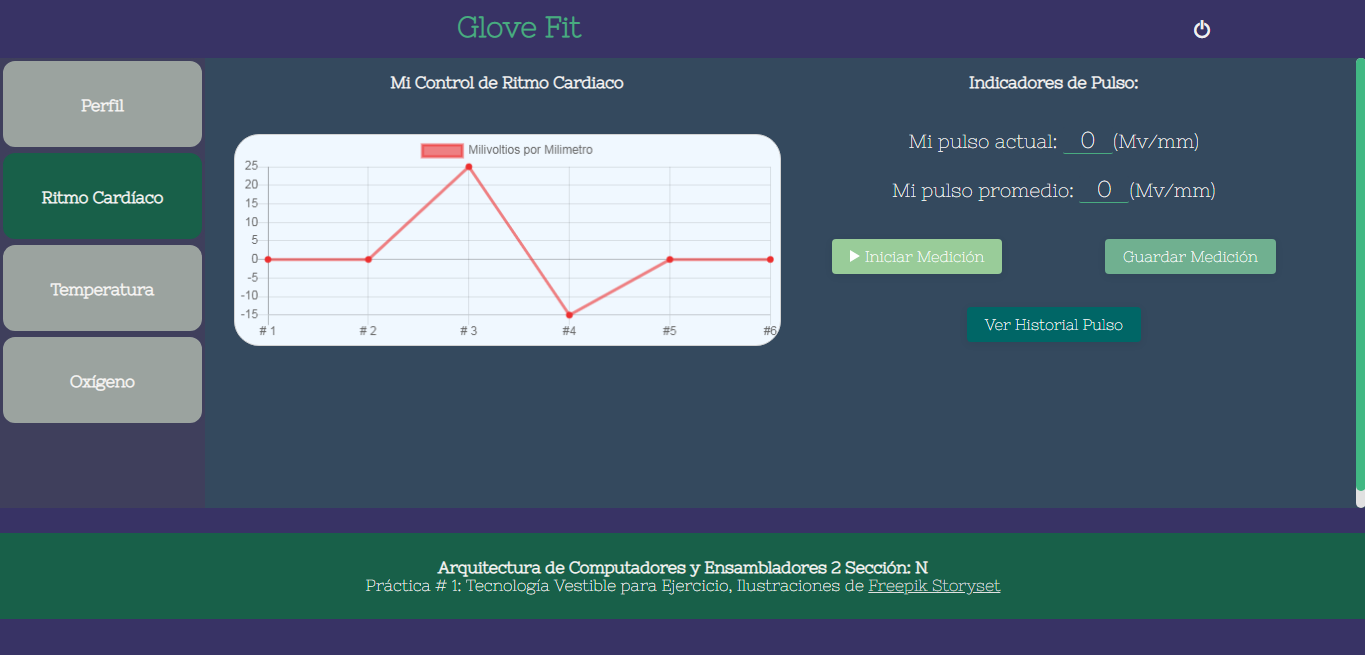
\includegraphics[width=0.45\textwidth]{RitmoC.PNG}
\end{figure}

    Con la ayuda de la opción "ver historial" es posible visualizar todas las sesiones de actividad física que el usuario ha realizado hasta el momento y dentro de cada sección los datos del pulso que se han recolectado.
    
\begin{figure} [H] \centering 
\caption{Figura 7: Historial Ritmo Cardiaco ( Página WEB )}
\includegraphics[width=0.45\textwidth]{RitmoCh.PNG}
\end{figure}

\subsubsection{Temperatura:}
    En esta sección es posible visualizar el control de la temperatura corporal del usuario en tiempo real.
    
\begin{figure} [H] \centering 
\caption{Figura 8: Temperatura ( Página WEB )}
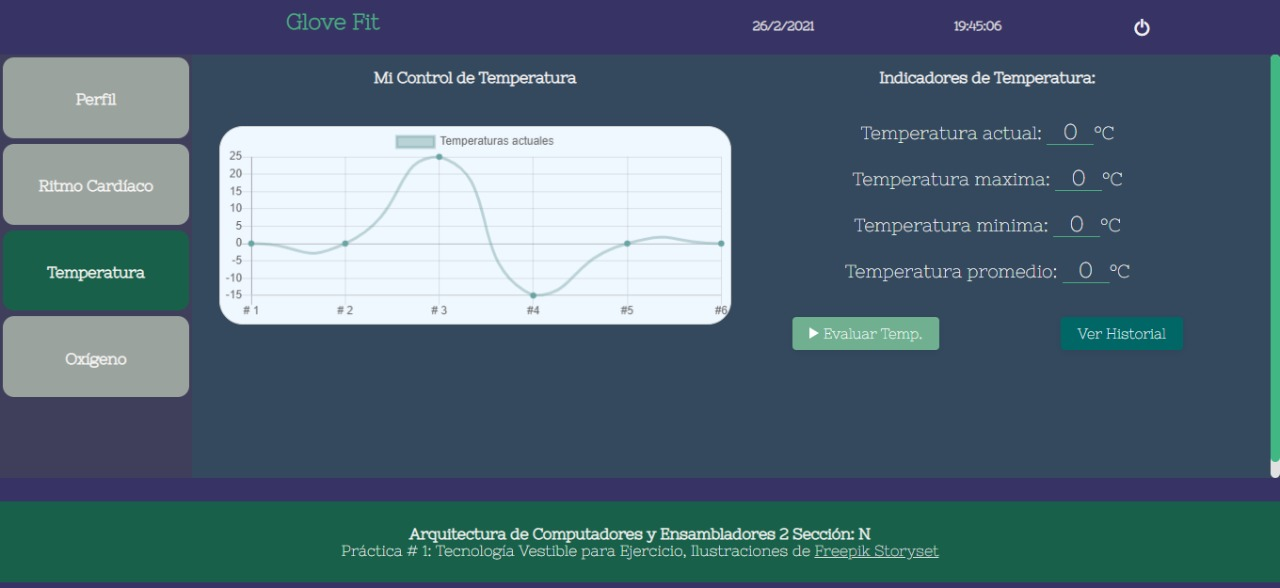
\includegraphics[width=0.45\textwidth]{temp.jpg}
\end{figure}

\subsubsection{Oxigeno:}
    En esta seccion se muestra el control del oxigeno en tiempo real.
    
\begin{figure} [H] \centering 
\caption{Figura 9: Oxigeno ( Página WEB )}
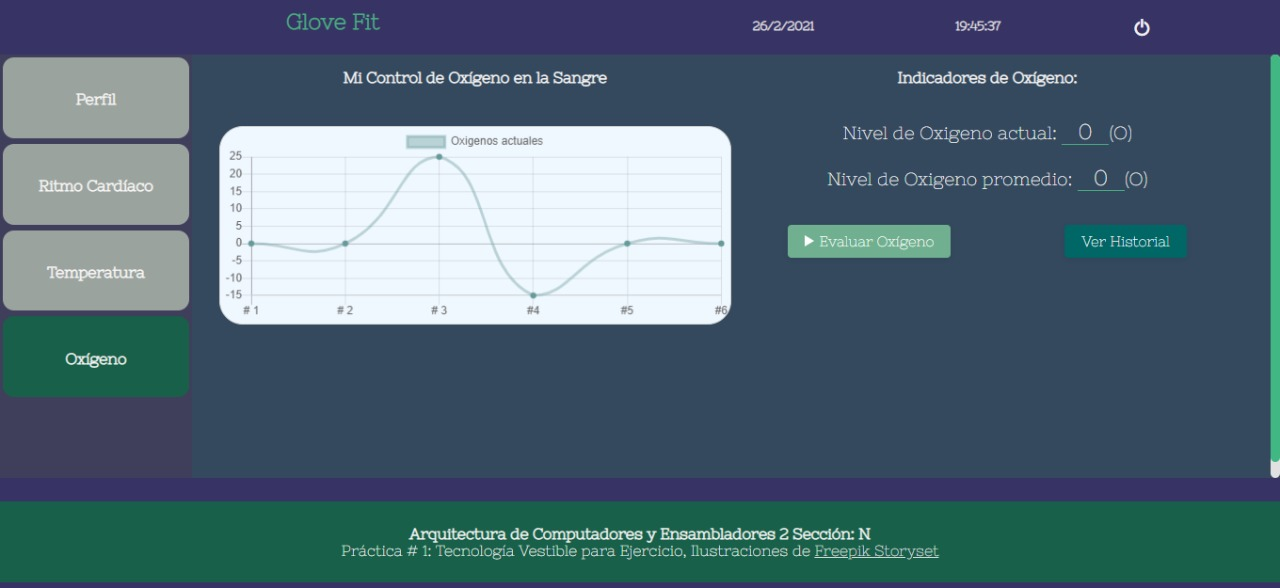
\includegraphics[width=0.45\textwidth]{oxig.jpg}
\end{figure}


    Con la opcion "ver historial" se muestran todos los datos que se han recolectado de la temperatura, pulso y oxigeno del usuario al momento de estar realizando una secion.
    
\begin{figure} [H] \centering 
\caption{Figura 9: Historial Rutina ( Página WEB )}
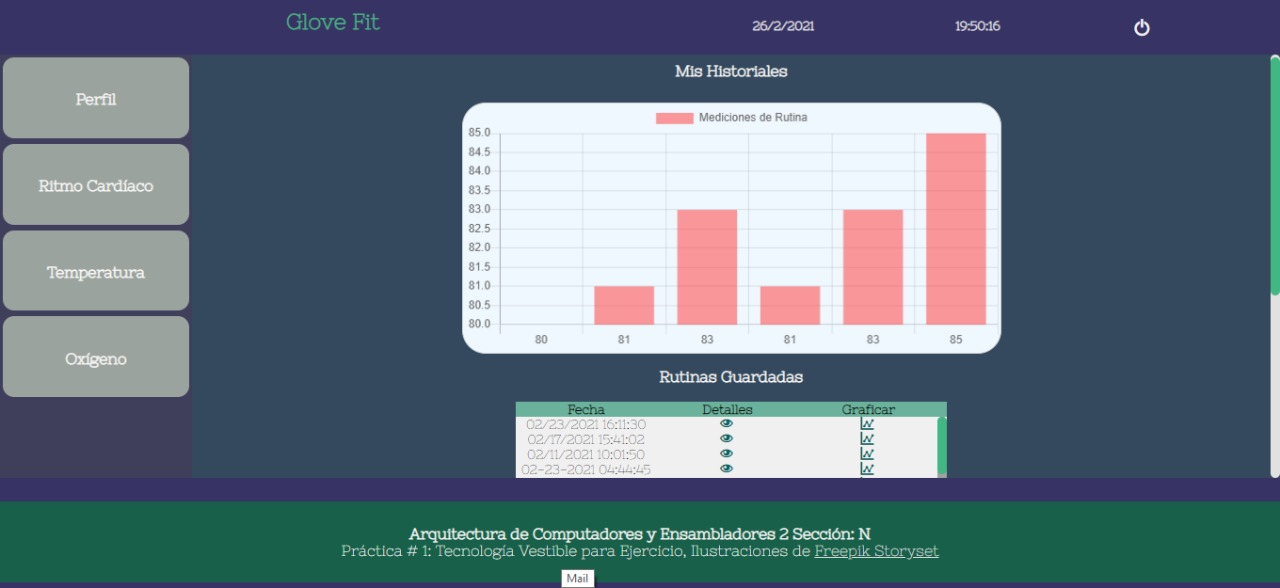
\includegraphics[width=0.45\textwidth]{hist.jpg}
\end{figure}

    El usuario coach puede seguir las rutinas de los atletas asignados y observar sus historiales
    
\begin{figure} [H] \centering 
\caption{Figura 10: Visualización de rutinas por parte de un Coach ( Página WEB )}
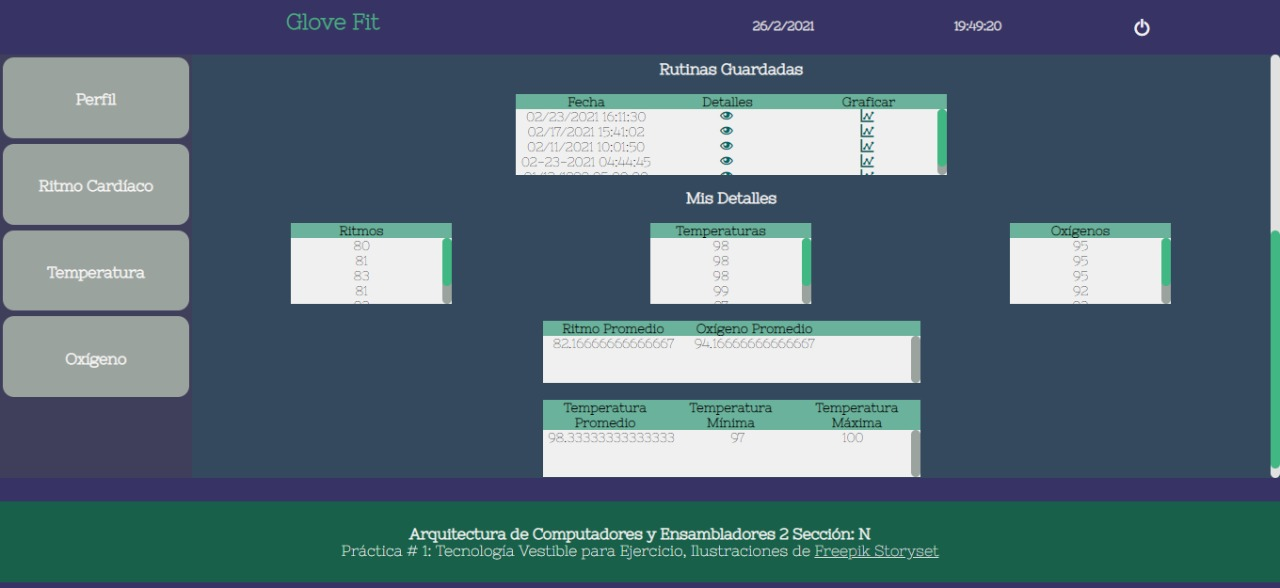
\includegraphics[width=0.45\textwidth]{HistAtle.jpg}
\end{figure}

\begin{figure} [H] \centering 
\caption{Figura 11: Visualización de atletas asignados a un coach ( Página WEB )}
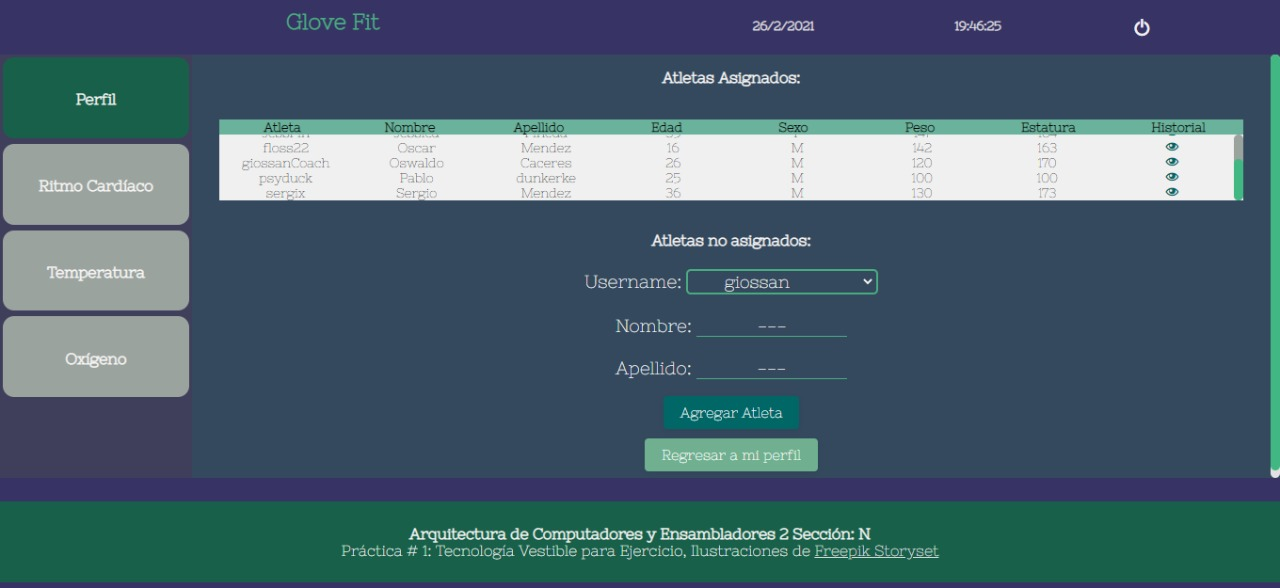
\includegraphics[width=0.45\textwidth]{AsigAtle.jpg}
\end{figure}



\section{Repositorio de Versiones: Git-Hub}
\href{https://github.com/airton47/ACE2_1S21_G15.git}{Repositorio de proyectos de grupo-15 \newline}
\newline
\url{https://github.com/airton47/ACE2_1S21_G15.git}



\end{document}